\documentclass{llncs}

\usepackage{microtype}
\usepackage{xspace}
\usepackage{booktabs}
\usepackage{todonotes}
\usepackage{wrapfig}
\newcommand{\KeY}{Ke\kern-1ptY\xspace}

\title{The \KeY Approach on Hagrid
  \\{\small VerifyThis Long-Term Challenge 2020 }}

\author{ Stijn de Gouw \and Mattias Ulbrich \and Alexander Weigl }
\institute{Open University \and Karlsruhe Institute of Technology}
\begin{document}
\maketitle

\section{Introduction}

In this report we present the applied \KeY approach on the VerifyThis Long Term
challenge 2020. Subject of the challenge was the HAGRID key server, a new
implementation of the PGP server to make the key server conform to
GDPR and resilient against DoS attacks.

% 1. Motivation
% 2. VerifyThis Challenge LTC
% 3. Verification target


\subsection{Introduction of the \KeY tool}

In its over 20 years of history, the \KeY-tool~\cite{KeyBook2} brings deductive
verification to Java Programs with support for fully Java 1.4 and JavaCard
\todo{version number} standard.
%
The calculi behind \KeY is based on the sequent calculi, and provides a sound
and (relative) complete reasoning on Java programs. This reasoning requires that
user-defined formal specification written in Java Modeling Language~\cite{Jml}.


\section{Verification Subject}

\KeY supports Java and is not applicable on Rust source code; so
re-implementation of HAGRID in Java was required. In summary we create two
different Java implementation: The first version uses only primitive data types
and arrays. In the second version, we modularize the first version to use a map
implementation. Both version are an abstraction of HAGRID as we focus on the
database logic. In the implementation, we avoid the use of objects: The e-mail
addresses and the keys are represented by integers. This also excludes the
parsing of PGP keys and also excludes the handling of HTTP protocol.

\paragraph{A simple email-key map.}

The most basic version is a simplified implementation for the keyserver --
verifiable without interactions in KeY, based on five integer arrays that store
for each user:
%
\begin{itemize}
  \item the id/email of the user, represented currently by an integer
  \item two arrays for confirmed and unconfirmed keys, and
  \item an array that stores confirmation codes.
  \item an array that stores which operation was most recently requested (the
    implementation only allows to confirm that operation)
\end{itemize}
%
The maximum number of users is fixed to 1024, as the arrays are never resized.
The table below shows the main metrics:

\begin{figure}
  \centering
  \begin{tabular}{ |c|c|c| }
    \hline
    Lines of Code & Lines of Specs & Proof Steps \\
    \hline
    69 & 82 & 30.119 \\
    \hline
  \end{tabular}
  \caption{Verification in numbers}
  \label{fig:numbers}
\end{figure}
% proof stats:
% addConfirm: 2665+2549
% addRequest: 5710
% delConfirm: 8321+2480
% delRequest: 2478+1212
% get: 1830
% posOfId: 2874


We also attempted to add a `timeout' mechanism, to cover the following aspect of the challenge:
\begin{quote}
  If the provided code \emph{is one recently issued} then the corresponding operation (addition/removal) is finalised
\end{quote}
This is easy to add in the implementation: first store the time that the user requests the operation (in an additional array), and when confirming, only approve the operation if that time was sufficiently recent. But it is problematic for specification and verification: the timelimit may not yet have elapsed in the precondition (i.e. the specification), but it may have when the JVM determines the current time in the \verb|confirm| method body.
So we dropped the timeout aspect.

\paragraph{Map version}

\begin{wrapfigure}[16]{R}{.5\textwidth}
  \centering
  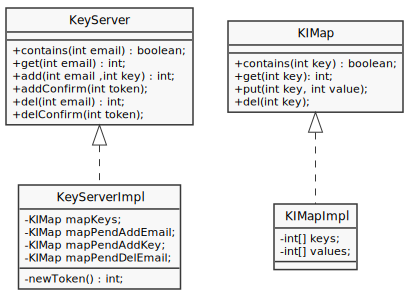
\includegraphics[width=.5\textwidth]{uml}
  \caption{UML class diagram of the Map version}
  \label{fig:umlclassdiagram}
\end{wrapfigure}
%
The next version builds upon the generalization of the previous map structure.
It is currently work in progress. This is a two-step process. The first step is
a provable version using maps of int to int. This avoids working with the heap.

KIMap (Key Integer Map) is an interface representing a map of Int to Int. This
functionality is bound to the behaviour of the map data type in KeY by JML
specification. KIMapImpl is a simple implementation based upon two int arrays,
one for the key, the other the values. KeyServerInt is a version of the backend
of the verifying key server using integers as e-mail addresses and keys. The
second step is to use Strings. This results into KSMap and KSMapImpl and also
the KeyServerString.
%

\iffalse
@startuml
skinparam monochrome true
skinparam shadowing false

class KeyServer {
    +contains(int email) : boolean;
    +get(int email) : int;
    +add(int email ,int key) : int;
    +addConfirm(int token);
    +del(int email) : int;
    +delConfirm(int token);
}

class KeyServerImpl implements KeyServer {
    -KIMap mapKeys;
    -KIMap mapPendAddEmail;
    -KIMap mapPendAddKey;
    -KIMap mapPendDelEmail;
    -newToken() : int;
}

class KIMap {
    +contains(int key) : boolean;
    +get(int key): int;
    +put(int key, int value);
    +del(int key);

}

class KIMapImpl implements KIMap {
}
@enduml
\fi

\section{Proofed Properties}

what has been achieved (modelled and verified properties)


\section{Conclusion }

% .. successes and challenges encountered in the course of the case study.

During the verification with \KeY we found some deficiencies: proving of heap
dependent stuffs.

\end{document}
